     \documentclass[a4paper,12p]{article}
\usepackage[utf8]{inputenc}
\usepackage[ngerman]{babel}
\usepackage[a4paper, left=2.5cm, right=2.5cm]{geometry}
\usepackage{amsmath}
\usepackage{graphicx}
\usepackage{mathtools}
\usepackage{tikz}
\usetikzlibrary{intersections}
\usetikzlibrary{calc,arrows.meta}  

\title{\huge Modellbildung\\\large \huge Beispielsammlung}
\author{\huge 4.Semester ET-Studium}
\date{\huge November 2018}
\begin{document}	
\maketitle
\newpage
\tableofcontents
\newpage
\section{Einleitung}
Die Modellbildung beschäftigt sich mit der mathematischen Beschreibung von Systemen, um diese dann beispielsweise mit Hilfe eines Reglers zu automatisieren.
\newline
Der Inhalt dieser Ausarbeitung beinhaltet nur die Aufgaben, aus dem Skript der Vorlesung der Modellbildung, welche eine Pflichtlehrveranstaltung im 4.Semester im Bachelor-Studium der Elektrotechnik ist. Der Lösungsweg der hier erwähnten Beispiele wird im Skript nicht explizit ausgearbeitet. Variablen der Form \textbf{x} sind Vektoren und der Form \textbf{A} sind Matrizen. \\
Die Ausarbeitung enthält nur die Beispiele die ohne nötiger Hilfe von Maple gelöst werden können und wo man keine mathematischen Beweise durchführen muss. \\
Außerdem beinhaltet dieses Dokument weiters komplett durchgerechnete Prüfungen.
\section{Mechanische Systeme}
\subsection{Punkt-Kinematik}
\textbf{\textit{\underline{Aufgabe 2.1}}}
\newline\newline
 Zeigen Sie, dass sich die Geschwindigkeitskomponenten eines materiellen Punktes \textit{P} im Raum bezüglich der normierten Basisvektoren $ e_{r} , e_{\theta} $ und $ e_{\varphi} $ in Kugelkoordinaten
 \begin{equation*}
 	x = r\sin(\theta)\cos(\varphi),\qquad y = r\sin(\theta)\sin(\varphi),\qquad z = r\cos(\theta)
 \end{equation*}
 zu
 \begin{equation*}
 	v_{r} = \dot{r},\qquad v_{\theta} = r\dot{\theta},\qquad v_{\varphi} = r\sin(\theta)\dot{\varphi}
 \end{equation*}
 errechnen.
 \newline\newline
 \textbf{Lösungsweg:}
 \newline\newline
 Die Geschwindigkeit mit der Form
 \begin{equation*}
 	\textbf{v}_{t} = v_{x}\textbf{e}_{x} + v_{y}\textbf{e}_{y} + v_{z}\textbf{e}_{z} = \dot{x}\textbf{e}_{x} + \dot{y}\textbf{e}_{y} + \dot{z}\textbf{e}_{z}
 \end{equation*}
 erhält man, durch die Anwendung der Kettenregel der Differentiation hier mit der Form
 \begin{equation*}
 	\textbf{v}(t) = \left(\frac{\partial}{\partial r}\textbf{r}\right) \dot{r} \ + \ \left(\frac{\partial}{\partial \varphi}\textbf{r}\right)  \dot{\varphi} \ + \ \left(\frac{\partial}{\partial \theta}\textbf{r}\right)\dot{\theta}
 \end{equation*}
 Die Basisvektoren bilden sich folgendermaßen aus
 \begin{align*}
 	\tilde{\textbf{e}}_{r} & = \sin(\theta)\cos(\varphi)\textbf{e}_{x} \ + \ \sin(\theta)\sin(\varphi)\textbf{e}_{y} \ + \ \cos(\theta)\textbf{e}_{z} \\ 
 	\tilde{\textbf{e}}_{\theta} & = r\cos(\theta)\cos(\varphi)\textbf{e}_{x} \ + \ r\cos(\theta)\sin(\varphi)\textbf{e}_{y} \ - \ r\sin(\theta)\textbf{e}_{z} \\
 	\tilde{\textbf{e}}_{\varphi} & = -r\sin(\theta)\sin(\varphi)\textbf{e}_{x} \ + \ r\sin(\theta)\cos(\varphi)\textbf{e}_{y} 	
 \end{align*}
 Diese Vektoren können nur dann eine zulässige Basis eines Koordinatensystems sein, wenn die Matrix
\begin{equation*}
	\textbf{J} =
	 \begin{bmatrix}
	 	\sin(\theta)\cos(\varphi) & \sin(\theta)\sin(\varphi) & \cos(\theta) \\
	 	r\cos(\theta)\cos(\varphi) & r\cos(\theta)\sin(\varphi) & -r\sin(\theta) \\
	 	-r\sin(\theta)\sin(\varphi) & r\sin(\theta)\cos(\varphi) & 0
	 \end{bmatrix}
\end{equation*}
\\
regulär ist. D.h. die Determinante dieser Matrix muss $\neq 0$  sein.
Die Matrix \textbf{J} wird folgendermaßen gefüllt: \\
\begin{equation*}
	\textbf{J} = 
		\begin{bmatrix}
			x_r & y_r & z_r \\
			x_\theta & y_\theta & z_\theta \\
			x_\varphi & y_\varphi & z_\varphi \\
		\end{bmatrix}
\end{equation*}
Hier det(\textbf{J}) = $r\sin\theta \neq 0$ wenn $r \neq 0$ und es gilt $\theta: [0,\frac{\pi}{2}]$ $\Rightarrow$ det(\textbf{J}) $\in$ regulär.\\
\underline{Beweis:} \\
Da es sich hier um eine $ 3 \times 3 $-Matrix handelt kann die Determinante dieser Matrix mithilfe des Satzes von Sarus gelöst werden.
\begin{align*}
	det(\textbf{J}) & = r^2\sin^3(\theta)\sin^2(\varphi) + r^2\cos^2(\theta)\cos^2(\varphi)\sin(\theta) + r^2\cos^2(\theta)\sin^2(\varphi)\sin(\theta) + r^2\sin^3(\theta)\cos^2(\varphi) =\\
	& = r^2(\sin^3(\theta)\sin^2(\varphi) + \cos^2(\theta)\cos^2(\varphi)\sin(\theta) + \cos^2(\theta)\sin^2(\varphi)\sin(\theta) + \sin^3(\theta)\cos^2(\varphi)) =\\
	& = r^2(\cos^2(\theta)\cos^2(\varphi)\sin(\theta) + \cos^2(\theta)\sin^2(\varphi)\sin(\theta) + \sin^3(\theta)(\sin^2(\varphi) + \cos^2(\varphi)) =\\
	& = r^2(\cos^2(\theta)\cos^2(\varphi)\sin(\theta) + \cos^2(\theta)\sin^2(\varphi)\sin(\theta) + \sin^3(\theta)) =\\
	& = r^2(\sin^3(\theta) + \cos^2(\theta)\sin(\theta)(\cos^2(\varphi) + \sin^2(\varphi))) =\\
	& = r^2(\sin^3(\theta) + \cos^2(\theta)\sin(\theta)) =\\
	& = r^2(\sin(\theta)\sin^2(\theta) + \cos^2(\theta)\sin(\theta)) = \\
	& = r^2(\sin(\theta)(\sin^2(\theta) + \cos^2(\theta))) = \\
	& = r^2\sin(\theta) \\ \\
	det(\textbf{J}) & = r^2\sin(\theta)
\end{align*}
Anschließend muss man die gerade ermittelten Basisvektoren normieren.\newline
Die Längen der Vektoren $\tilde{\textbf{e}}_{r},\tilde{\textbf{e}}_{\varphi}$ und $\tilde{\textbf{e}}_{\theta}$ betragen $1,r\sin\theta$ und $r$.
\newline
Normierte Basisvektoren:
\begin{align*}
	\textbf{e}_{r} & = \sin(\theta)\cos(\varphi)\textbf{e}_{x} \ + \ \sin\theta)\sin(\varphi)\textbf{e}_{y} \ + \ \cos(\theta)\textbf{e}_{z} \\
	\textbf{e}_{\theta} & = \cos(\theta)\cos(\varphi)\textbf{e}_{x} \ + \ \cos(\theta)\sin(\varphi)\textbf{e}_{y} \ - \sin(\theta)\textbf{e}_{z} \\
	\textbf{e}_{\varphi} & = -\sin(\varphi)\textbf{e}_{x} \ + \ \cos(\varphi)\textbf{e}_{y}
\end{align*}
Mit diesen Basisvektoren lässt sich die Geschwindigkeit in der Form
\begin{equation*}
	\textbf{v}(t) = v_{r}\textbf{e}_{r} + v_{\theta}\textbf{e}_{\theta} + v_{\varphi}\textbf{e}_{\varphi} = \dot{r}\textbf{e}_{r} + r\dot{\theta}\textbf{e}_{\theta} +  r\sin(\theta)\dot{\varphi}\textbf{e}_{\varphi}
\end{equation*}
darstellen.
\begin{equation*}
	v_r = \dot{r} \ , \ v_\theta = r\dot{\theta} \ , \ v_\varphi = r\sin(\theta)\dot{\varphi}
\end{equation*}
\newpage
\subsection{Newtonsche Gesetze}
\subsubsection{Kräftesystem}
\textbf{\textit{\underline{Aufgabe 2.3}}} \\ \\
Ein vertikaler Mast M wird gemäß der Abbildung durch Seile abgespannt.
\begin{figure}[h]
\begin{center}
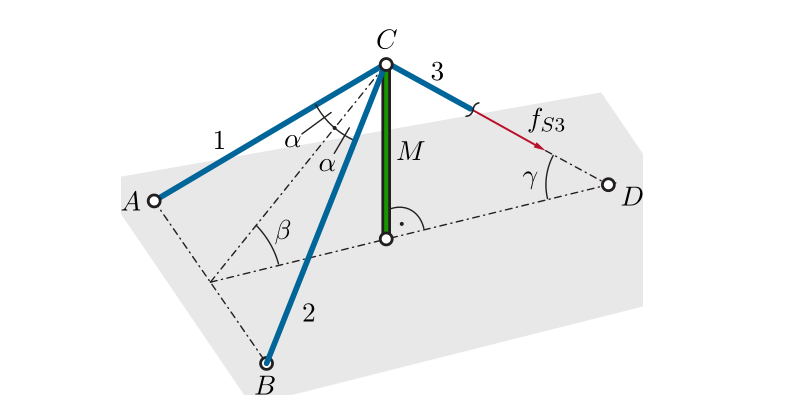
\includegraphics[width=12.5cm]{pic/Angabe}
\caption{Angabe Aufgabe 2.3}
\label{Angabe}
\end{center}
\end{figure} \\
Wie groß sind die Kräfte $ f_{s1} $ und $ f_{s2} $ in den Seilen 1 und 2 und die Kraft $ f_M $ im Mast, wenn am Seil 3 die Zugkraft $ f_{s3} $ aufgebracht wird? \\ \\
\textbf{Lösungsweg:} \\ \\
Zunächst müssen die Gleichungen für die Gleichgewichtsbedingung aufgestellt werden. Da sich es in Abbildung \ref{Angabe} um ein 3-dimensionales Beispiel handelt muss man die Gleichgewichtsbedingung für alle drei Raumrichtungen aufstellen.
\begin{align*}
	(1) \ \ \ e_x & : f_{s1}\cos(\alpha) - f_{s2}\cos(\alpha) = 0 \\
	(2) \ \ \ e_y & : f_{s3}\cos(\gamma) - f_{s1}\cos(\alpha)\cos(\beta) - f_{s2}\cos(\alpha)\cos(\beta) = 0 \\  
	(3) \ \ \ e_z & : -f_M - f_{s3}\sin(\gamma) - f_{s2}\cos(\alpha)\sin(\beta) - f_{s1}\cos(\alpha)\sin(\beta) = 0
\end{align*}
Nun hat man ein einfaches Gleichungssystem mit 3 Gleichungen, welches nach diesen auch gelöst werden soll. Als erstes formt man die Gleichung (1) auf $f_{s1}$ um. \\ 
Hieraus folgt:
\begin{equation*}
	f_{s1} = f_{s2}
\end{equation*}
Im nächsten Schritt setzt man die umgeformte Gleichung (1) in Gleichung (2) ein und formt diese auf $ f_{s1} $ um. \\
Hieraus folgt:
\begin{align*}
	f_{s3}&\cos(\gamma) - f_{s1}\cos(\alpha)\cos(\beta) - f_{s1}\cos(\alpha)\cos(\beta) = 0 \\
	f_{s3}&\cos(\gamma) - 2f_{s1}\cos(\alpha)\cos(\beta) = 0 \\
	f_{s1}&=f_{s2} = \frac{f_{s3}\cos(\gamma)}{2\cos(\alpha)\cos(\beta)}
\end{align*}

\begin{flushleft}
    \textbf{\textit{\underline{Aufgabe 2.4}}}
\end{flushleft}
Geben Sie die Momentenbilanz für das Beispiel von Abbildung 2.14 um den Bezugspunkt \textit{C} an.  \newline
\begin{figure}[h]
    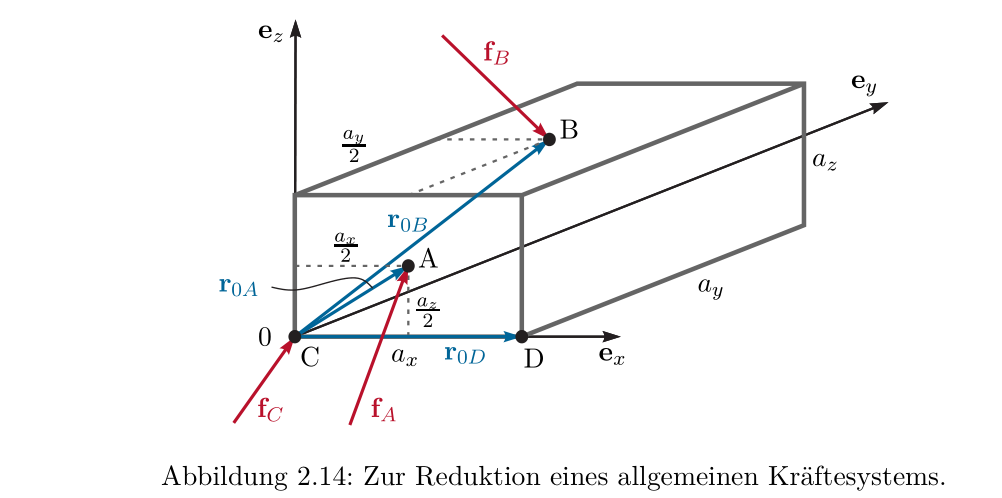
\includegraphics[width=12.5cm]{pic/Angabe2_4}
    \caption{Angabe Aufgabe 2.4}
    \label{Angabe 2.4}
\end{figure}
\begin{flushleft}
Ausgehend von den Kräften
\end{flushleft}
\begin{equation*}
	\textbf{f}_{A} = \left[\begin{array}{c}	f_{A,x} \\	f_{A,y} \\	f_{A,z} \\\end{array}\right] , 
	\textbf{f}_{B} = \left[\begin{array}{c}	f_{B,x} \\	f_{B,y} \\	f_{B,z} \\\end{array}\right] ,
	\textbf{f}_{C} = \left[\begin{array}{c}	f_{C,x} \\	f_{C,y} \\	f_{C,z} \\\end{array}\right]
\end{equation*}
sowie die zugehörigen Ortsvektoren
\begin{equation*}
	\textbf{r}_{0A} = \left[\begin{array}{c} \frac{a_{x}}{2} \\ 0 \\ \frac{a_{z}}{2} \\\end{array}\right] ,
	\textbf{r}_{0B} = \left[\begin{array}{c} \frac{a_{x}}{2} \\ \frac{a_{y}}{2} \\ a_{z} \\\end{array}\right]
	\textbf{r}_{0C} = \left[\begin{array}{c} 0 \\ 0 \\ 0 \\\end{array}\right]
	\textbf{r}_{0D} = \left[\begin{array}{c} a_{x} \\ 0 \\ 0 \\\end{array}\right]
\end{equation*}
\newpage
\begin{flushleft}
	Für den Bezugspunkt \textit{C} folgen die Momente zu
\end{flushleft}
\begin{align*}
	\boldsymbol{\tau}_{A}^{(C)} &= \underbrace{(\textbf{r}_{0A} - \textbf{r}_{0C})}_{\textbf{r}_{CA}} \times \textbf{f}_{A} = \left[\begin{array}{c} \frac{a_{x}}{2} \\ 0 \\ \frac{a_{z}}{2} \\\end{array}\right] \times \left[\begin{array}{c} f_{A,x} \\ f_{A,y} \\ f_{A,z} \\\end{array}\right] = \left[\begin{array}{c}
		-\frac{f_{A,y}a_{z}}{2} \\
		-\frac{f_{A,z}a_{x}}{2} + \frac{f_{a,x}a_{z}}{2} \\
		\frac{f_{A,y}a_{x}}{2} \\
	\end{array}\right]
	\\
	\boldsymbol{\tau}_{B}^{(C)} &= \underbrace{(\textbf{r}_{0B} - \textbf{r}_{0C})}_{\textbf{r}_{CB}} \times \textbf{f}_{B} = 
	\left[\begin{array}{c}
		\frac{a_{x}}{2} \\
		\frac{a_{y}}{2} \\
		a_{z} \\
	\end{array}\right]
	\times
	\left[
	\begin{array}{c}
		f_{B,x} \\
		f_{B,y} \\
		f_{B,z} \\
	\end{array}
	\right]
	=
	\left[\begin{array}{c}
	\frac{f_{B,y}a_{z}}{2} - f_{B,y}a_{z} \\
	-\frac{f_{B,z}a_{x}}{2} + f_{B,x}a_{z} \\
	\frac{f_{B,y}a_{x}}{2} - \frac{f_{B,x}a_{y}}{2} \\
	\end{array}\right]
	\\
	\boldsymbol{\tau}_{C}^{(C)} &= \underbrace{(\textbf{r}_{0C} - \textbf{r}_{0C})}_{\textbf{r}_{CC}} \times \textbf{f}_{C} = 
	\left[\begin{array}{c}
			0 \\
			0 \\
			0 \\
	\end{array}\right]
	\times
	\left[
	\begin{array}{c}
	f_{C,x} \\
	f_{C,y} \\
	f_{C,z} \\
	\end{array}
	\right]
	=
	\left[\begin{array}{c}
		0 \\
		0 \\
		0 \\
	\end{array}\right]
\end{align*}
\subsubsection{Schwerpunkt}
\begin{flushleft}
	\underline{\textbf{\textit{Aufgabe 2.6}}} \\
\end{flushleft}
Berechnen Sie den Schwerpunkt einer homogenen Halbkugel gemäß Abbildung 2.19. 
\begin{figure}[h]
	\begin{center}
		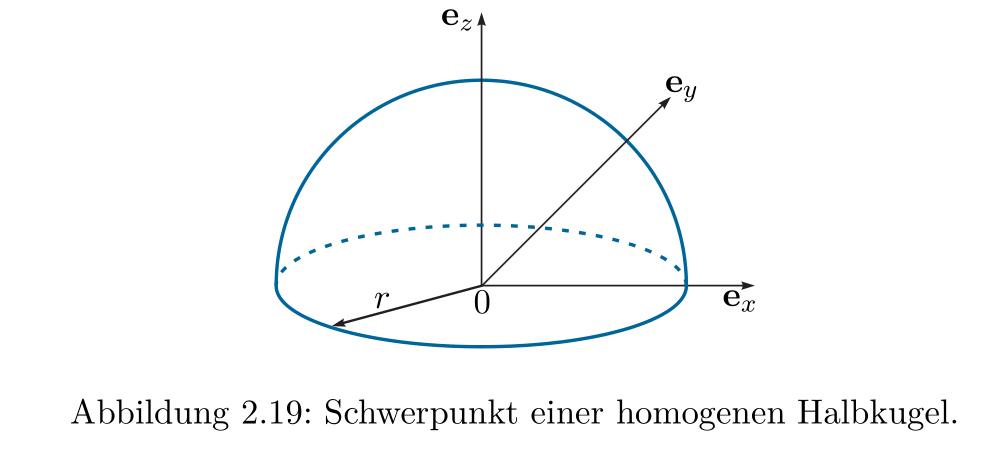
\includegraphics[width=12.5cm]{pic/Angabe2_6}
		\caption{Angabe Aufgabe 2.6}
		\label{Aufgabe2.6}
	\end{center}
\end{figure} 
\newline
\textbf{Lösungsweg:} \\
Schwerpunkt einer homogenen Halbkugel: \\
\begin{align*}
	dV &= \int_{0}^{2\pi}\int_{0}^{\frac{\pi}{2}}\int_{0}^{r}R^2\sin(\theta)dr d\theta d\varphi = \\
	dV &= \frac{2r^3\pi}{3}
\end{align*}
\newpage
Koordinaten des Ortsvektors zum Schwerpunkt:
\begin{align*}
	r_{Sx} &= \int_{0}^{2\pi}\int_{0}^{\frac{\pi}{2}}\int_{0}^{r}r^3\sin(\theta)\cos(\varphi)\sin(\theta)dr d\theta d\varphi = 0 \\
	r_{Sy} &= \int_{0}^{2\pi}\int_{0}^{\frac{\pi}{2}}\int_{0}^{r}r^3\sin(\theta)\sin(\varphi)\sin(\theta)dr d\theta d\varphi = 0 \\
	r_{Sz} &= \int_{0}^{2\pi}\int_{0}^{\frac{\pi}{2}}\int_{0}^{r}r^3\cos(\theta)\sin(\theta)dr d\theta d\varphi = \frac{\pi r^4}{4}
\end{align*}
Koordinaten als Vektor:
\[
	\textbf{r}_{SK} = 
	\left[
		\begin{array}{c}
			0 \\
			0 \\
		    \frac{\pi r^4}{4} \\
		\end{array}
	\right]
\]
Schwerpunkt:
\[
	\textbf{r}_{S} = \frac{\textbf{r}_{SK}}{dV} = 
	\left[
		\begin{array}{c}
			0 \\
			0 \\
			\frac{3}{8}r \\
		\end{array}
	\right]
\]
\subsubsection{Impulserhaltung}
Die Aufgaben in diesem Kapitel beinhalten nur Beweise, aber diese Ausarbeitung behandelt keine mathematischen Beweise.
\subsubsection{Translatorische kinetische Energie und potentielle Energie  }
\underline{\textbf{\textit{Aufgabe 2.9}}} \\ \\
Berechnen Sie jeweils die Gesamtsteifigkeit $c_{g}$ sowie die zugehörige entspannte Länge $s_{0g}$ der Ersatzschaltung gemäß der Angabe.
\begin{figure}[h]
	\begin{center}
		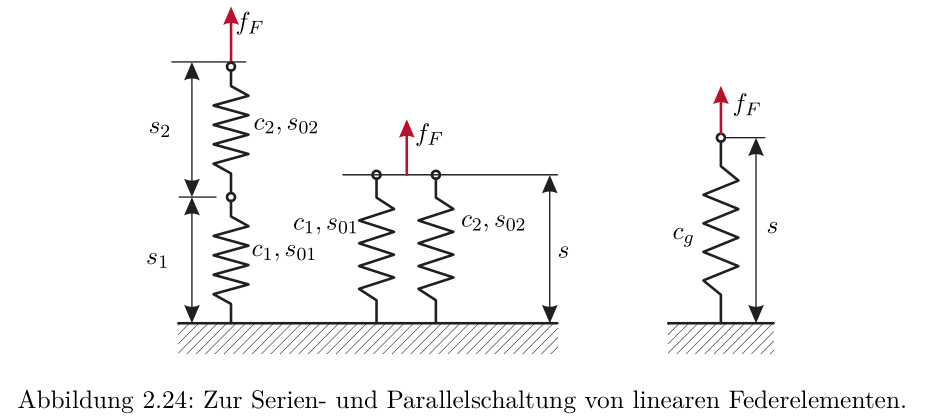
\includegraphics[width=12.5cm]{pic/Angabe2_9}
		\caption{Angabe Augfabe 2.9}
		\label{Aufgabe 2.9}
	\end{center}
\end{figure}
\newpage
\begin{flushleft}
	\textbf{Lösungsweg:}
\end{flushleft}
Serienschaltung:\\
Die entspannten Längen werde addiert und die Steifigkeit wird wie einer einer "Parallelschaltung" berechnet.
\[
	s_{0g} = s_{10} + s_{20}, \qquad c_{g} = \frac{c_{1}c_{2}}{c_{1} + c_{2}}
\]
\begin{flushleft}
Parallelschaltung:
\end{flushleft}
Steifigkeit:
\[ c_{g} = c_{1} + c_{2}\]
entspannte Länge:
\begin{align*}
	feder1_{F0} &= c_{1}s_{10} \\
	feder2_{F0} &= c_{2}s_{20} \\
	F_{g0} = feder1_{F0} + feder2_{F0} &= c_{1}s_{10} + c_{2}s_{20} \\
	s_{g0} = \frac{F_{g0}}{c_{g}} &= \frac{c_{1}s_{10} + c_{2}s_{20}}{c_{1} + c_{2}}
\end{align*}
\subsubsection{Dissipative Kräfte }
\underline{\textbf{\textit{Aufgabe 2.10}}}\\ \\
Berechnen Sie die notwendige Zugkraft $f_{s}$ als Funktion der Winkel $\alpha$ und $\beta$ sowie der Masse $m$ und des Haftreibungskoeffizienten $\mu_{H}$, damit die Masse bewegt werden kann.
\begin{figure}[h]
	\begin{center}
		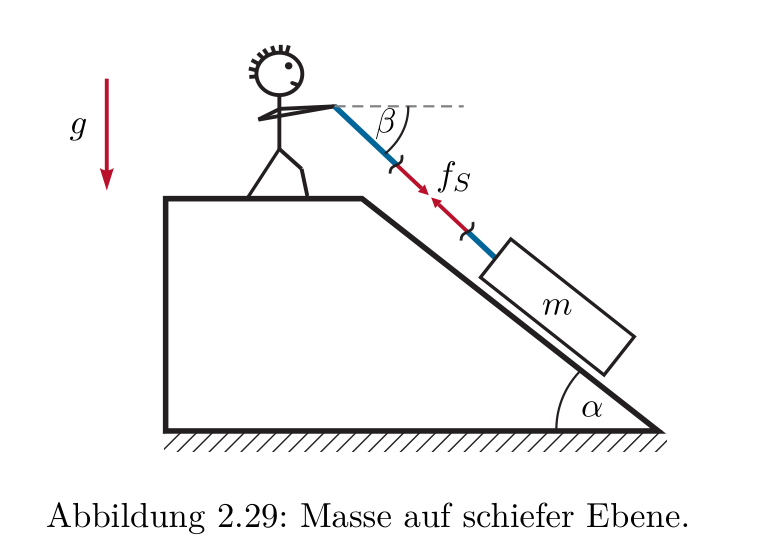
\includegraphics[width=10    cm]{pic/Angabe2_10}
		\caption{Angabe Aufgabe 2.10}
		\label{Angabe 2.10}
	\end{center}
\end{figure}
\newpage
\begin{flushleft}
	\textbf{Lösungsweg:}
\end{flushleft}
\begin{figure}[h]
	\begin{center}
		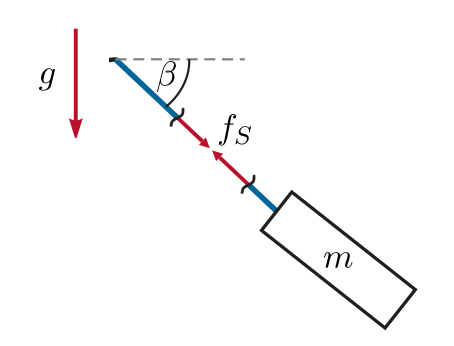
\includegraphics[width=7.5cm]{pic/Angabe2_10_2}
		\caption{Freigeschnittener Masseblock}
		\label{Loesung2.10}
	\end{center}
\end{figure}
Gleichgewichtsbedingungen:
\begin{align*}
	\textbf{e}_{x} &: -f_{s}\cos(\beta) + f_{R}\cos(\alpha) + f_{N}\sin(\alpha) = 0 \\
	\textbf{e}_{y} &: -mg + f_{s}\sin(\beta) - f_{r}\sin(\alpha) + f_{N}\cos(\alpha) = 0 \\
\end{align*}
Haftreibungskraft $f_{R} = f_{N}\mu_{H}$ \\
Setzt man diese in die obigen Bedingungen lässt sich folgendes Gleichungssystem ermitteln: \\
$\textbf{e}_{x}:$
\begin{align*}
	 -f_{S}\cos(\beta) + f_{N}\mu_{H}\cos(\alpha) + f_{N}\sin(\alpha) = 0 \\
	 -f_{S}\cos(\beta) + f_{N}(\mu_{H}\cos(\alpha) + \sin(\alpha)) = 0 \\
\end{align*}
$\textbf{e}_{y}:$
\begin{align*}
	-mg + f_{S}\sin(\beta) - f_{N}\mu_{H}\sin(\beta) + f_{N}\cos(\alpha) = 0 \\
	-mg + f_{S}\sin(\beta) - f_{N}(\mu_{H}\sin(\alpha) + \cos(\alpha)) = 0 \\
\end{align*}
Gleichungssystem:
\begin{align*}
	I  &: -f_{S}\cos(\beta) + f_{N}(\mu_{H}\cos(\alpha) + \sin(\alpha)) = 0 \\
	II &: 	-mg + f_{S}\sin(\beta) - f_{N}(\mu_{H}\sin(\alpha) + \cos(\alpha)) = 0 \\
\end{align*}
Nun wird ganz normal dieses Gleichungssystem gelöst.\\
I auf $f_{N}$ umgeformt:
\[
	f_{N} = \frac{f_{S}\cos(\beta)}{\mu_{H}\cos(\alpha) + \sin(\alpha)}
\]
I in II eingesetzt und auf $f_{S}$ umgeformt:
\begin{align*}
	&-mg + f_{S}\sin(\beta) - \frac{f_{S}\cos(\beta)}{\mu_{H}\cos(\alpha) + \sin(\alpha)}(\mu_{H}\sin(\alpha) + \cos(\alpha)) = 0 \\
	&-mg(\mu_{H}\cos(\alpha) + \sin(\alpha)) + f_{S}\sin(\beta)(\mu_{H}\cos(\alpha) + \sin(\alpha)) - f_{S}\cos(\beta)(\mu_{H}\sin(\alpha) + \cos(\alpha)) = 0 \\
	&-mg(\mu_{H}\cos(\alpha) + \sin(\alpha)) + f_{S}(\mu_{H}\sin(\beta)\cos(\alpha) + \sin(\beta)\sin(\alpha)) - f_{S}(\mu_{H}\cos(\beta)\sin(\alpha) + \cos(\alpha)\cos(\beta)) = 0 \\
	&-mg(\mu_{H}\cos(\alpha) + \sin(\alpha)) + f_{S}(\mu_{H}\underbrace{(\sin(\beta)\cos(\alpha) - \cos(\beta)\sin(\alpha))}_{\sin(\beta - \alpha)} + \underbrace{(\sin(\beta)\sin(\alpha) + \cos(\beta)\cos(\alpha))}_{\cos(\beta - \alpha)}) = 0 \\
	&-mg(\mu_{H}\cos(\alpha) + \sin(\alpha)) + f_{S}(\mu_{H}\sin(\beta - \alpha) + \cos(\beta - \alpha)) = 0 \\
	&f_{S} = \frac{mg(\mu_{H}\cos(\alpha) + \sin(\alpha))}{\cos(\beta - \alpha) + \mu_{H}\sin(\beta - \alpha)}
\end{align*}
\newline
Der Körper haftet bei der Bedingung \( |f_{S}|\leq f_{H}\).\\
Damit der Körper sich nun bewegen kann muss \(|f_{S}| > f_{H}\) erfüllt. Daraus folgt für \(f_{S}\):
\[
	f_{S} > \frac{mg(\mu_{H}\cos(\alpha) + \sin(\alpha))}{\cos(\beta - \alpha) + \mu_{H}\sin(\beta - \alpha)}
\] 

\section{Wärmeübertragung}
\textbf{Cross-String-Methode:} \\
Dies ist eine Berechnungsmethode für die Sichtfaktormatrix 2-dimensionaler Geometrien. Mit dem folgendem Beispiel wird nun erklärt wie man diese Methode genau verwendet. \\


\renewcommand\thesection{\Alph{section}} % Umstellung des Section-Zählung auf Buchstaben
\setcounter{section}{1} % Damit die neue Section bei B beginnt
\section{Aufgaben zum Selbststudium}
Sämtliche Angaben zu diesem Beispielen finden Sie im Skript dieser Lehrveranstaltung. Diese Zusammenfassung soll die Lösungen aus dem Skript vereinfachen.
\newpage
\subsection{Klappbrücke}
Anfangs werden der Träger und die Brücke einmal frei geschnitten. \\ \\
\begin{figure}[h]
\begin{center}
	\begin{tikzpicture}[scale=1.5]
	\draw[green!50!black,thick]
	(0.25,0.75) -- (3.14,1.52) -- +(0.15,-0.45) -- (0.5,0.33);
	\draw[thick]
	(0,0.5) -- (0,0) -- (0.5,0) -- +(0,0.5);
	\draw[thick]
	(0.25,0.75) arc (90:0:0.25cm);
	\draw[thick]
	(0.25,0.75) arc (90:180:0.25cm);
	\draw[dashed]
	(0.25,0.5) -- +(15:3.125cm);
	\draw[thick]
	(0.25,0.5) circle (3pt);
	\draw[-Latex,thick]
	(-0.5,0.5) node[below]{$f_{Bx}$} -- (0.25,0.5);
	\draw[-Latex,thick]
	(0.25,-0.5) node[right]{$f_{By}$} -- (0.25,0.5);
	\draw[-Latex,thick]
	(1.75,0.90) -- +(0,-1) node[right]{$m_Bg$};
	\fill
		(1.75,0.9) circle (1pt);
	\draw[-Latex,thick]
	(2.66,1.14) -- +(0,1) node[right]{$f_{s1}$};
	\fill
		(2.66,1.14) circle (1pt);
	\draw[very thin]
		(0.25,0.5) -- +(2.5,0);
	\draw[very thin,-Latex]
		(2.7,0.5) node[right] {$\varphi_B$}  arc (0:18.5:2cm);
	\end{tikzpicture}
	\caption{freigeschnittene Brücke}
\end{center}
\end{figure}

\\ Gleichgewichtsbedingungen:
\begin{align*}
	\textbf{e}_{x} &: f_{B,x} = 0 \\
	\textbf{e}_{y} &: f_{B,y} - m_Bg + f_{s1} = 0 \\
	\textbf{e}_{z} &: -m_Bgl_B\cos\varphi_B  + f_{s1}l_s\cos\varphi_B = 0
\end{align*}
\end{document}